% politeness cogsci submission


\documentclass[10pt,letterpaper]{article}

\usepackage{cogsci}
\usepackage{pslatex}
\usepackage{color}
 \newcommand{\denote}[1]{\mbox{ $[\![ #1 ]\!]$}}
\definecolor{Red}{RGB}{255,0,0}
\newcommand{\red}[1]{\textcolor{Red}{#1}}  
\usepackage[nodoi]{apacite}
\usepackage{graphicx}
\usepackage[american]{babel}
\usepackage{amsmath}
\usepackage[section]{placeins}
\usepackage{enumitem}
\usepackage{apacite}


\title{An integrative account of politeness: 
Reasoning about communicative informativity and kindness}
 
\author{{\large \bf Erica J. Yoon} \\
  \texttt{ejyoon@stanford.edu} \\
  Department of Psychology \\
  Stanford University
  \And {\large \bf Michael Henry Tessler} \\
  \texttt{mtessler@stanford.edu} \\
  Department of Psychology \\
  Stanford University
  \And {\large \bf Noah D. Goodman} \\
  \texttt{ngoodman@stanford.edu} \\
  Department of Psychology \\
  Stanford University
  \And {\large \bf Michael C. Frank} \\
  \texttt{mcfrank@stanford.edu} \\
  Department of Psychology \\
  Stanford University}

\begin{document}

\maketitle


\begin{abstract}

...

\textbf{Keywords:} 
Politeness; computational modeling; communicative goals; pragmatics

\end{abstract}


\section{Introduction}

Imagine that Alice just gave a presentation, and asked Bob for his opinion, who thought the presentation was terrible. Bob decides to say to Alice: ``Your talk was okay.''

In the situation above, Bob faces a dilemma: on one hand, he would want to give the most accurate information possible to Alice, but on the other hand, by directly telling her the truth, Bob would make Alice feel bad, and Bob might lose his own reputation of being a person with good intentions.This scenario represents what \citeA{Brown1987} identified as a \emph{face-threatening act} (FTA), which intrinsically threatens interactants' \emph{face}, or their positive self-image. 

Based on \citeA{Brown1987}'s model, there are at least two wants that the speaker has and must weigh: (a) communicate the content of the FTA (i.e., the true state of the world); (b) to save the listener's face. We revisit these ideas and posit that, in a situation where a speaker is called to remark on and evaluate the listener's performance, there are two kinds of goals a speaker has: (1) To be ``honest'' (vs. ``dishonest'): to convey the true state of the world as truthfully and accurately as possible (vs. to hide it); (2) To be ``nice'' (vs. ``mean''): to make the listener feel good about themselves and save the listener's face (vs. to make them feel bad and lose face)

% Note the difference between honesty/truthfulness as determined before vs. after the intended informational content is  decided?

Previous research has linked politeness with honesty, but as a personality trait rather than a strategy connected to the idea of informativity. Bonnefon et al. (2009) found that people find an utterance such as ``some people hated your poem?? as less honest but nicer when actually ``all?? people hated it. Follow-up study showed that people who think of themselves as honest interpret an ambiguous utterance in a way that is more informative but face-threatening (Feeney and Bonnefon, 2013). The interpretation was that individual differences in personality characteristics contribute to pragmatic computation. In the current work, we argue that speakers reason about the relative weights for goals of honesty and kindness, and listeners account for speaker?s such goals and make inferences accordingly.

The current work empirically tests people's lay notion of politeness as a way to balance between conveying accurate information and saving the interactants' positive face (\emph{epistemic utility} and \emph{social utility} respectively; discussed in Computational Model section below). We also present a formal model of a listener to thinks about a speaker who considers both the goals of improving the knowledge state of the listener and making the listener feel good about him- or herself. 

% note about van roij's hypothesis about polite utterances as costly
% lee and pinker 2010: indirectness coming from cooperation AND conflict; but we argue for stronger bias toward thinking that people are cooperative (maximally informative and kind, as much as they can be)

\section{Computational Model}

Politeness poses a challenge for Gricean models of pragmatic language understanding, which assume that speakers' goals are to communicate informatively about some aspect of the world \cite{Frank2012, Goodman2013}. 
Why ever would you say \emph{please} or \emph{thank you} if they only add cost to the speaker and carry no information content?
Similarly, what incentive is there to ever ``sugar coat'' utterances if the only currency of communication is information transfer? 
We propose that information transfer captures just one component of a speaker's utility, \emph{epistemic utility}.
Politeness, then, takes shape as an independent component of a speaker's utility, what we will call \emph{social utility}. 

\citeA{Goodman2013} define speaker utility by the amount of information a \emph{literal listener} would still not know after know about world state $s$ after hearing a speaker's utterance $w$: 
$U_{epistemic}(w; s) = \ln(P_{literal}(s \mid w)) $.
We simply extend this by adding a component related to the intrinsic value of the state in the eye's of the listener\footnote{At this point, we do not differentiate value of the state to the listener from value of the state to the speaker, though it is conceivable that these could be different.}.
We consider states which have utility values 1 - 5, corresponding to the subjective utility of the state, and roughly corresponding to the scalar value terms \{\emph{good}, \emph{bad}, \emph{terrible}, \emph{amazing}, and \emph{okay}\}. 
The precise mapping from utterance to subjective utility value is measured in Expt.~1.

We define the social utility of an utterance to be the expected utility of the state the listener would infer given the utterance $w$: 
%
$$
U_{social}(w; s) = E_{V}[[P_{literal}(s \mid w)]]
$$
%
where $V$ is the value function that maps states to subjective utility values. 

Experiment 2 explores the relative contributions of these two utility components under a variety of scenarios. 
In order to consider the relative contributions of the two utility components, we transform both components to probability space (values between 0 - 1): $U_{epistemic}$ by exponentiating; $U_{social}$ by normalizing. Thus, the speaker's joint utility function is
%
$$
U(w;s; \beta) = \beta_{e}\cdot e^{U_{epistemic}} + \beta_{s} \cdot \frac{U_{social}}{\max_{s} V(s)}
$$
%
We follow the treatment of RSA using lifted-variables \cite{GoodmanLassiter2015, Kao2014, Degen2015}; here, the variables lifted to the pragmatic level are the weights in the speaker's utility function ($\beta$'s) .

%
\begin{eqnarray}
&&P_{L_1}(s, \beta \mid w)\propto P_{S_1}(w \mid s, \beta)\cdot P(s) \cdot P(\beta) \label{eq:L1}\\
&&P_{S_1}(w \mid s, \beta) \propto \mathrm{exp}(\lambda \cdot E[[U(w; s; \beta)]])\label{eq:S1}\\
&&P_{L_0}(s \mid w, \beta)\propto \denote{w}(s) \cdot P(s) \label{eq:L0}
\end{eqnarray}
%
For simplicity, we assume the following:
\begin{enumerate}
\item The set of states of the world $S = \{s_{1}, ...,  s_{5}\}$ have subjective numerical values $V(s_{i}) = i$. 
\item The set of utterances is \{\emph{amazing, bad, okay, good, amazing}\},
% $\{w_{amazing}, w_{bad}, w_{okay}, w_{good}, w_{amazing}\}$
  \red{used in relevant empirical studies \cite{Bonnefon} (?).}\end{enumerate}
 % these were used in Kao & Goodman (2015), should we cite it as being relevant though?
The literal meaning of these utterances $W$ with respect to states $S$ we measure in Expt.~1. 



\section{Behavioral Experiments}

We conducted three experiments to probe human data to look at: (1) literal semantics judgment: what utterance in its literal sense is perceived to aptly describe the true state of the world (i.e., speaker's true feelings toward the listener's performance; referred to as `true state' from here on); (2) goal inference: given the true state and the speaker's actual utterance to the listener, what goals are attributed to the speaker; (3) state inference: given the speaker's goal and utterance to the listener, what is the true state?

\subsection{Experiment 1: Literal semantics}

\subsubsection{Method}

We created 13 different context items, in which a person (e.g., Ann) gave a performance of some kind, and another person (e.g., Bob) evaluated it. For example, in one of the contexts, Ann baked a cake, and Bob tasted it. Bob's feelings toward Ann's cake (``\emph{true state}'') were shown on a scale out of five hearts (e.g., two out of five hearts filled in red color). Then we asked, ``Do you think Bob thought Ann's cake was X?'' where X could be one of five possible words: \emph{terrible}, \emph{bad}, \emph{okay}, \emph{good}, and \emph{amazing}.

30 participants with IP addresses in the United States were recruited on Amazon's Mechanical Turk. Each participant read 25 scenarios, depicting every possible combination of 5 true states and 5 words. Participants indicated their answer to each question by answering `No' or `Yes.' The order of context items was randomized, and there were a maximum of two repeats of each context item per participant.

\subsubsection{Results}

Perhaps as expected, negatively-connoted words were matched with the negative end states, and positively- connoted words with positive end states with the highest likelihood (see Figure \ref{fig:exp1}). The word ``terrible'' had its highest likelihood at state of one heart (``state 1'' from here on) and sharply decreased as state positivity increased. The word ``bad'' had its highest likelihood at state 1 and 2, then sharply decreased as state positivity increased. The words ``amazing'' and ``good'' followed a symmetric, opposite pattern of yielding the highest likelihoods at positive states and close-to-zero likelihoods at negative states. The word ``okay'' had its peak likelihood at state 3, and decreased as state moved away from being ‘neutral,' either negatively or positively.

\begin{figure*}[t]
\begin{center} 
  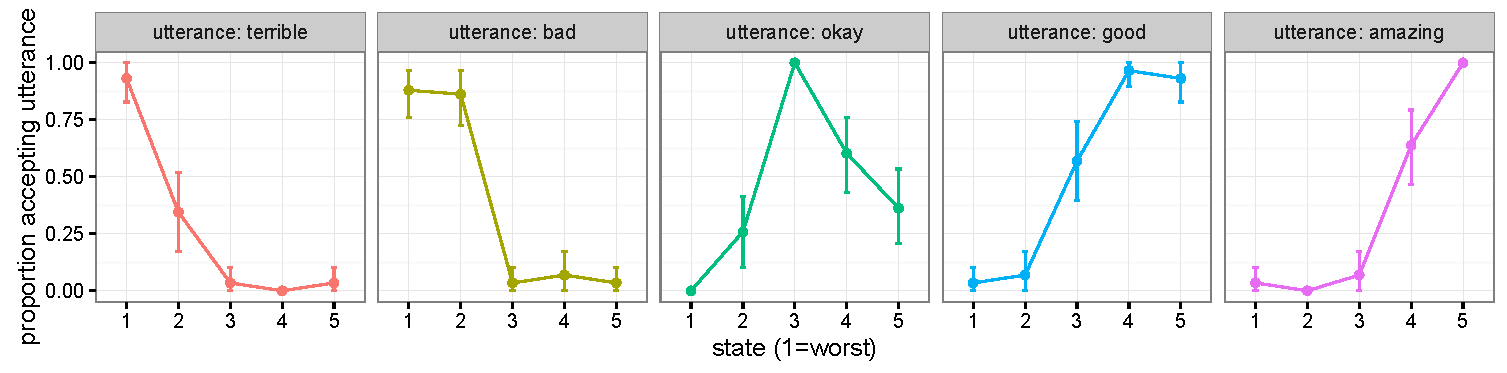
\includegraphics[width=.9\textwidth]{figures/exp1.pdf}
  \caption{\label{fig:exp1} Results from Experiment 1. Proportion of acceptances of words (shown in different colors) given the true state represented on a scale of hearts.}
  \end{center} 
\end{figure*}

\subsection{Experiment 2: Goal inference}

\subsubsection{Method} 

We presented scenarios in which a person (e.g., Ann) gave some performance and asked for another person (e.g., Bob)'s opinion on the performance. The same context items and true states as Experiment 1 were used. Additionally, we provided information on what Bob actually said to Ann (e.g., ``Your cake was okay''), where Bob used one of the five possible words,  \emph{terrible}, \emph{bad}, \emph{okay}, \emph{good}, and \emph{amazing}. Then we asked participants to infer the likelihood of Bob's goals to be honest, nice, and mean: the question read, ``Based on what Bob said, how likely do you think that Bob's goal was to be: honest; nice; mean,'' with the three goals placed in a random order below three slider bars, on which the participant could indicate each goal's likelihood.

\begin{figure*}[t]
\begin{center} 
  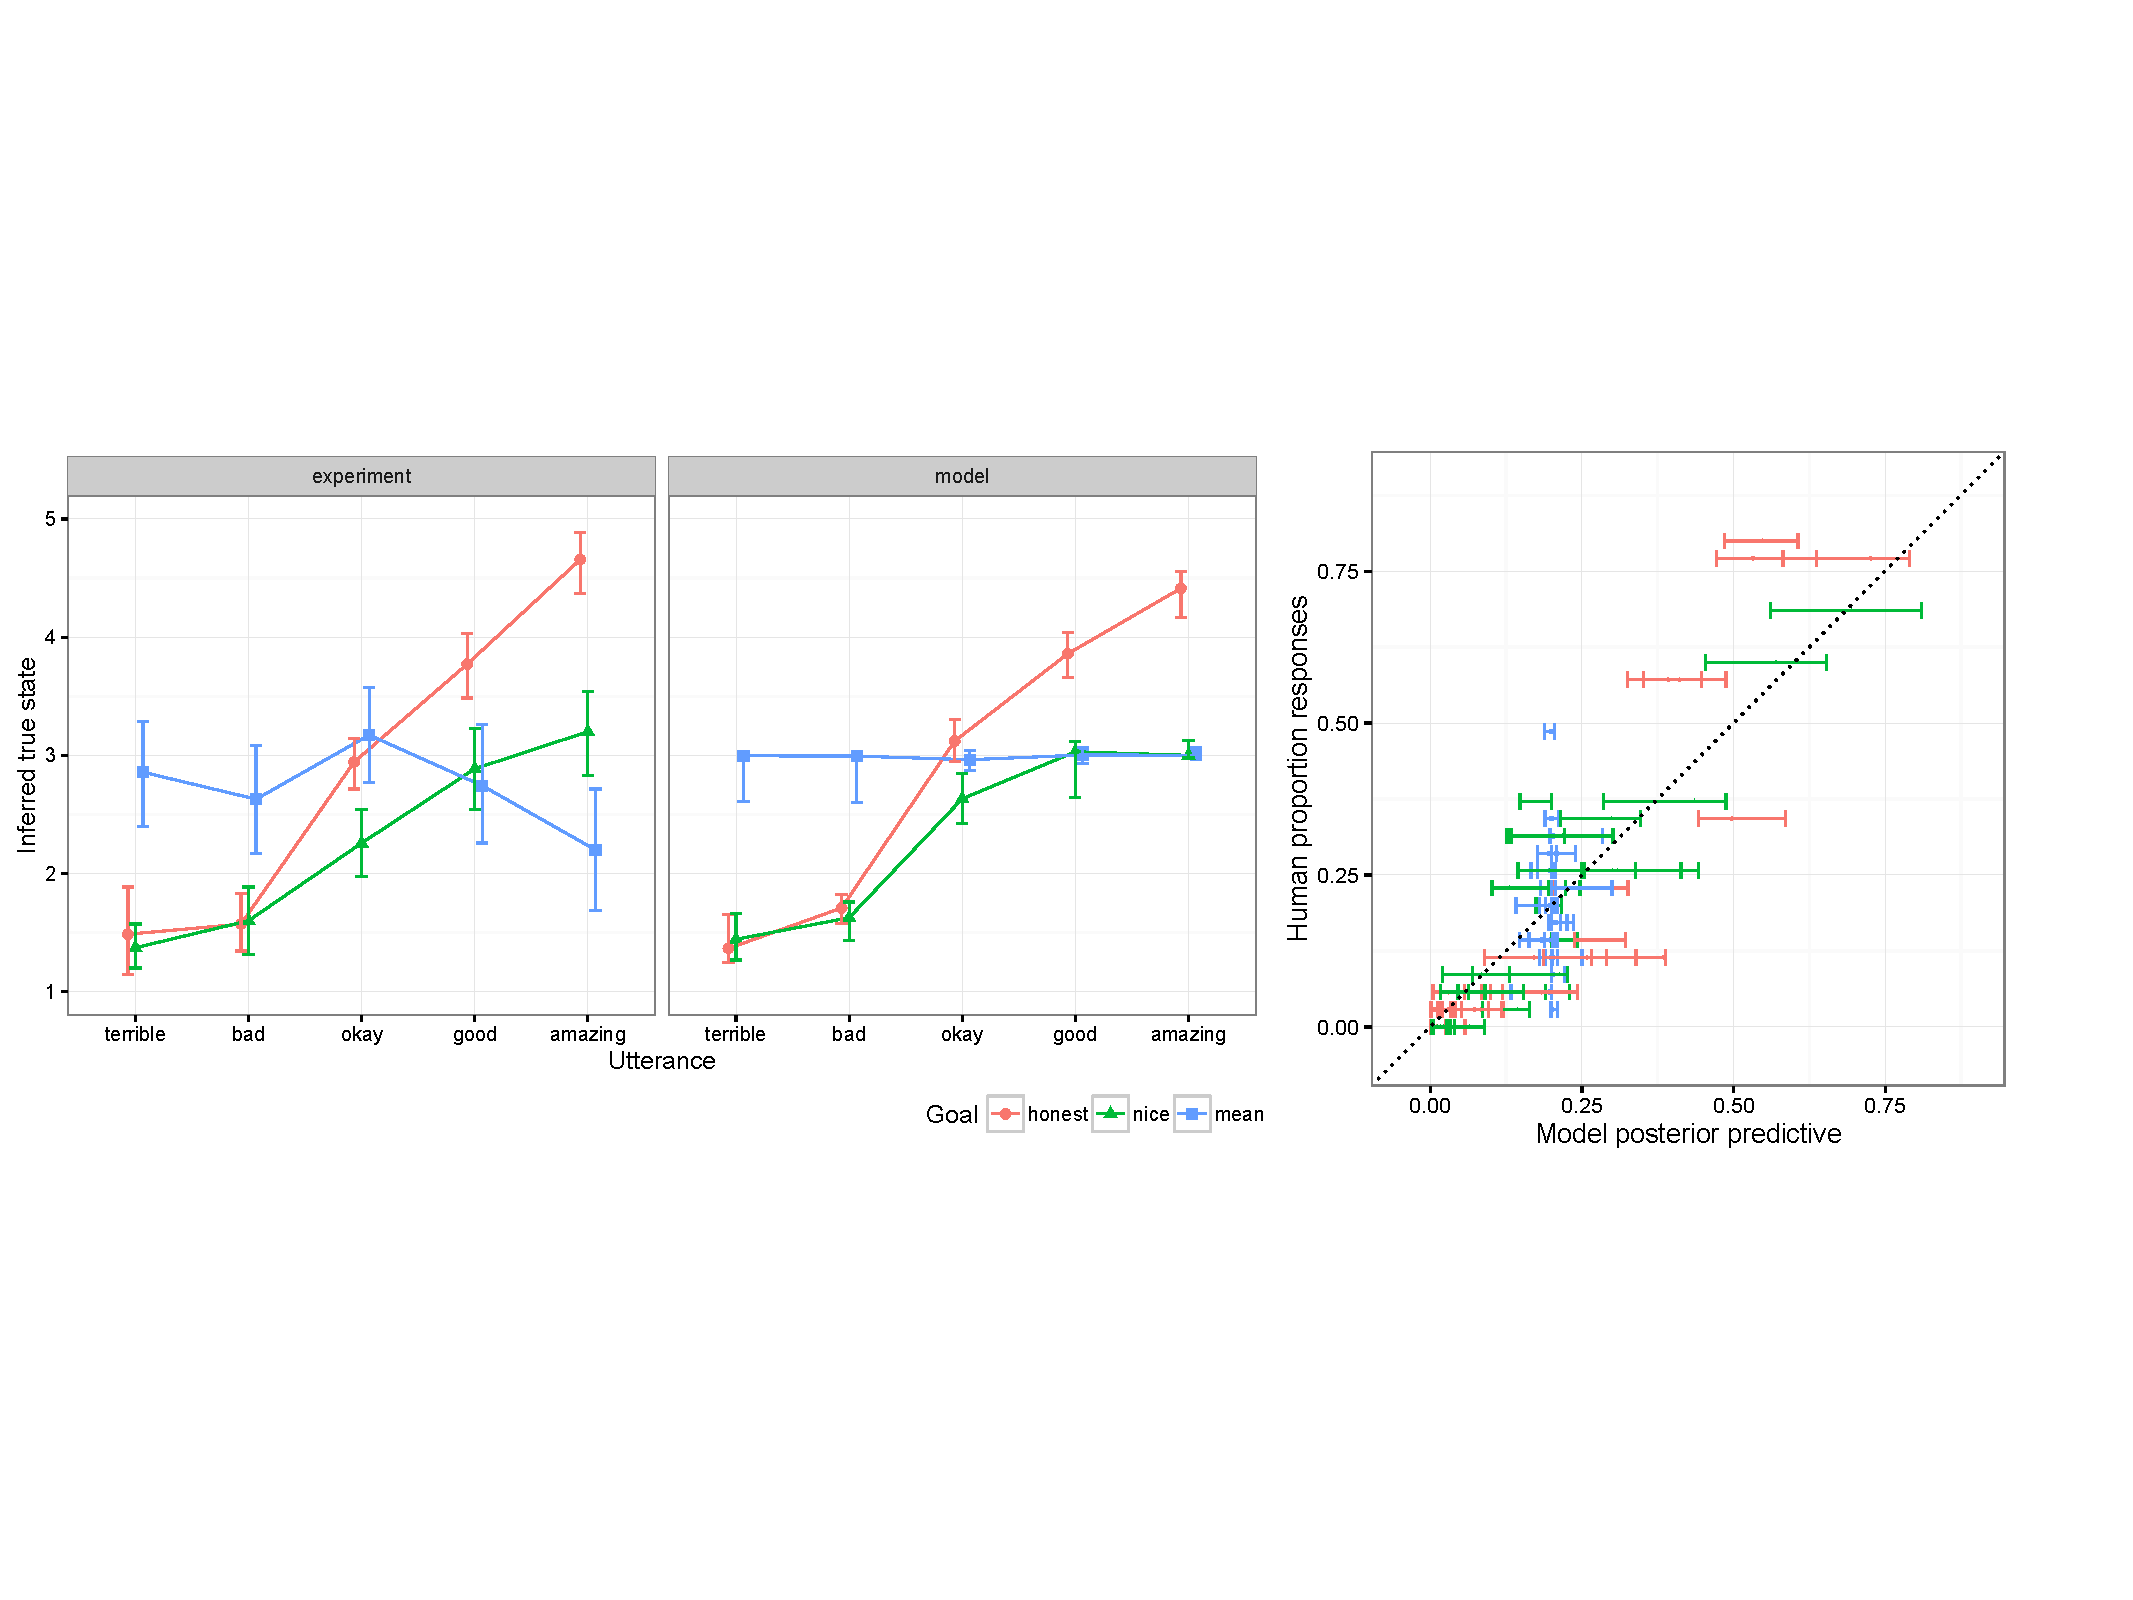
\includegraphics[width=.9\textwidth]{figures/exp2.pdf}
  \caption{\label{fig:exp2} Results from Experiment 2 (top) and model predictions (bottom). Attribution of speaker's goals (honest vs. nice vs. mean, shown in different colors) based on the true state and utterance.}
  \end{center} 
\end{figure*}


\subsubsection{Results}

Participants attributed likelihoods for speaker's goals differently depending on how closely the literal meaning of the utterance matched the true state (based on the distribution shown in Experiment 1). When the literal meaning of the utterance was close to the true state, participants attributed the goal to be honest with the highest likelihood (note the similarity between the honesty goal attribution and the literal semantics distribution). When the literal meaning of the utterance did not match the true state, people attributed a goal to be nice, if the utterance had a positive bias, or a goal to be mean, if the utterance had a negative bias.

There was an interesting asymmetry between niceness vs. meanness goal attribution, in that positive utterances are perceived to arise from niceness goal regardless of the state, whereas negative utterances are only perceived to be mean given a positive true state. This perhaps reflects participants' lay notion of an optimal speaker who tries to be kind and honest; speaker's critical remark (e.g., ``bad'') is perceived to be out of a good will to be maximally truthful to the listener, rather than intention to damage the listener's reputation.

Another interesting observation comes from judgments about the utterance ``[it was] okay.'' The niceness goal attribution decreases, and meanness goal attribution increases, as state positivity increases. That is, it was perceived to be unkind to say that an amazing presentation was ``okay,'' whereas the same utterance for a terrible presentation was perceived to be kind. This suggests that the meaning for ``okay'' is somewhat flexible, and is constructed relative to the given state.

\subsection{Experiment 3: State inference}

\subsubsection{Method}

The procedure was the same as Experiment 2, except that, instead of providing information on the speaker (e.g., Bob)'s utterance and feelings about a person (e.g., Ann)'s performance (\emph{true state}) and asking for inference on Bob's goals, we provided information on Bob's utterance and his \emph{goal} (e.g., the prompt read: ``Bob wanted to be nice: ``It was okay,'' he said''), and asked for participants' inference on the true state (i.e., Bob's true feelings about Ann's performance), which they indicated on a scale of five hearts.

\subsubsection{Results}

Given the speaker's goal to be honest, as predicted from the literal semantics distribution, inferred state positivity was correlated with utterance positivity: ``terrible'' implied approximately the true state of 1, ``okay'' the state of 3, ``amazing'' the state of 5. Interestingly, state inferred based on the utterance ``[It was] bad'' was not judged to be different from the inferred state based on ``terrible,'' which is seemingly more negatively-connoted. In contrast, the inferred state based on ``good'' was less positive than inferred based on ``amazing.'' This may suggest that saying even a weakly negative remark (e.g., ``bad'') is face-threatening to a similar degree as making a more strongly negative comment, given that the speaker has already decided to express criticism.

Given the speaker's goal to be nice, the inferred state positivity is also correlated with the utterance positivity, but participants inferred that the states are less positive compared to states given honesty goal, based on neutral and positive utterances. Based on the utterance ``amazing,'' participants inferred the true state to be close to 5 given the honesty goal, but they inferred the state to be around 3 given the niceness goal. Thus, participants reasoned that a speaker who is trying to be nice produced an utterance  with a literal meaning that is more positive that the speaker's true feelings toward the listener's performance.

It should be noted that more positive utterances lead to inference of more positive states given the goal to be nice, which indicates that people think a ``nice'' speaker is still being somewhat informative with respect to communicating what the true state is. Thus, a nice speaker probably used the word ``amazing'' to describe an okay presentation rather than a terrible one.

Curiously, inferred states based on honesty and niceness goals did not differ from each other given negative utterances (``terrible'' and ``bad''). %This could be due to a floor effect, arising from the limitation of the scale that is currently used to represent the true state, which does not provide an option for a state worse than ``terrible.'' Presumably, a speaker who is trying to be nice but ends up saying``terrible'' leads participants to think that the true state was the worst it could be, but the only way to indicate this on the heart scale was give the minimum number of hearts (``1'') which matches the literal meaning of ``terrible.''

Finally, given the speaker's goal to be mean, participants inferred that the true states were more positive if the speaker's utterance was negative or neutral. Thus, they judged that a mean speaker saying ``terrible'' meant it was not terrible but okay (state of 3). Interestingly, if a positive utterance was produced with the goal to be mean, the true state was inferred to be worse compared to the states based on honesty and niceness goal. That is, a mean speaker saying ``amazing'' was judged to mean that the state was worse than average. This may be due to irony in play: making an extremely positive remark about an extremely bad performance is perceived to be sarcastic and ill-intentioned \cite{colston1997}. Our current model does not include a component of sarcasm, and it will be useful addition in the future.

\begin{figure}
\begin{centering} 
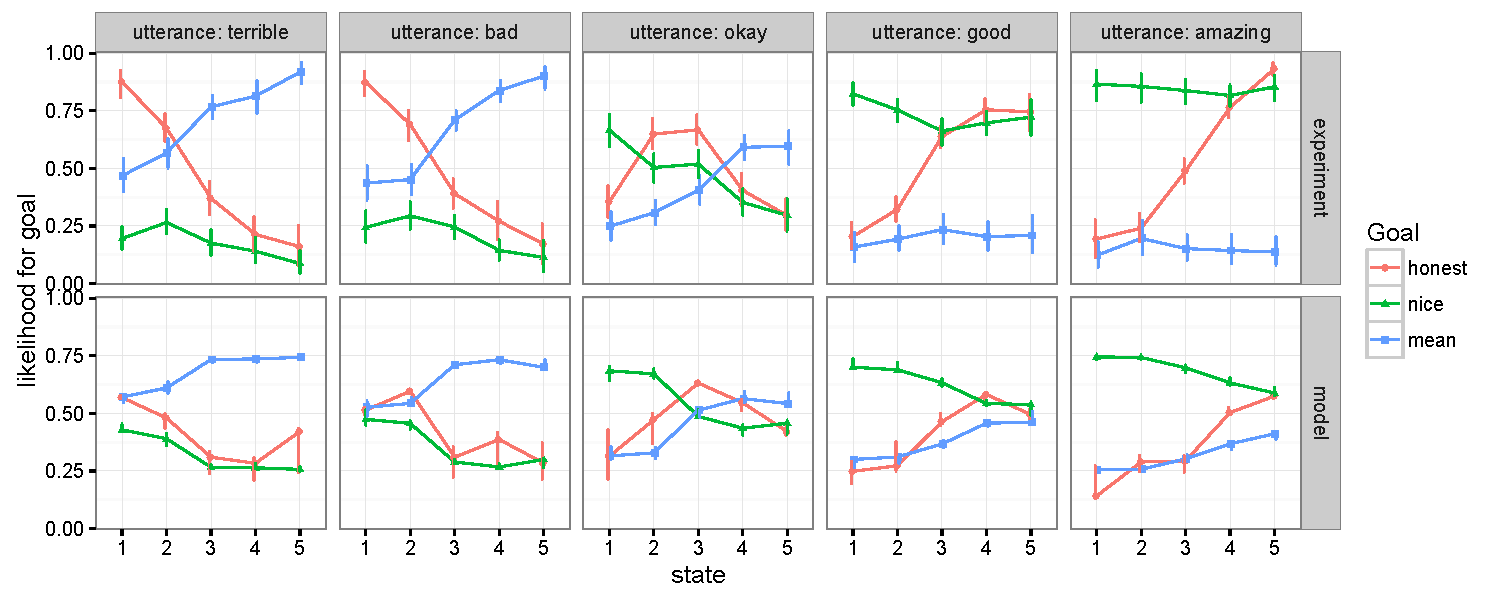
\includegraphics[width=3.2in]{figures/exp3.pdf}
\caption{\label{fig:exp3} Results from Experiment 3. Average states inferred based on speaker's goal and utterance.}
\end{centering} 
\end{figure}


\bibliographystyle{apacite}

\setlength{\bibleftmargin}{.125in}
\setlength{\bibindent}{-\bibleftmargin}

\bibliography{politeness}


\end{document}
